\chapter{Games}
Still has not passed enough time to implement Vulkan in a huge variety of games. But there are some companies that
have implement the \gls{api} for develop their engines.

The first company to launch a game supporting this \gls{api} has been \emph{Oxide Games} with the game \emph{Ashes of
Singularity}, a strategy on real time game. It has been the first game to support DirectX12 too. It is strange that
they have released the game under Windows, having the chance of supporting other platforms.

\emph{Doom}, is one of the first AAA games that implemented Vulkan a few months after it was put on sale. Normally,
\emph{ID Software}, the company that has developed this saga, has typically developed their games with the OpenGL
\gls{api}. In this case, they have develop the game using their engine ID Tech 6 - based on OpenGL - and then they
have added support to Vulkan with excellent results.

Valve has implemented Vulkan in their engine Source 2. So that games as \emph{Dota 2} have been the first titles to
offer multiplatform support. \emph{Ark: Survival Evolver} is other game offering multiplatform support with an
excellent quality.

Other videogame examples that implement Vulkan, in desktop as much in mobile devices, are \emph{Vainglory}
\ref{fig:vainglory}, \emph{Rust}, \emph{Need for Speed: No Limits}...

\begin{figure}[t]
	\begin{center}
		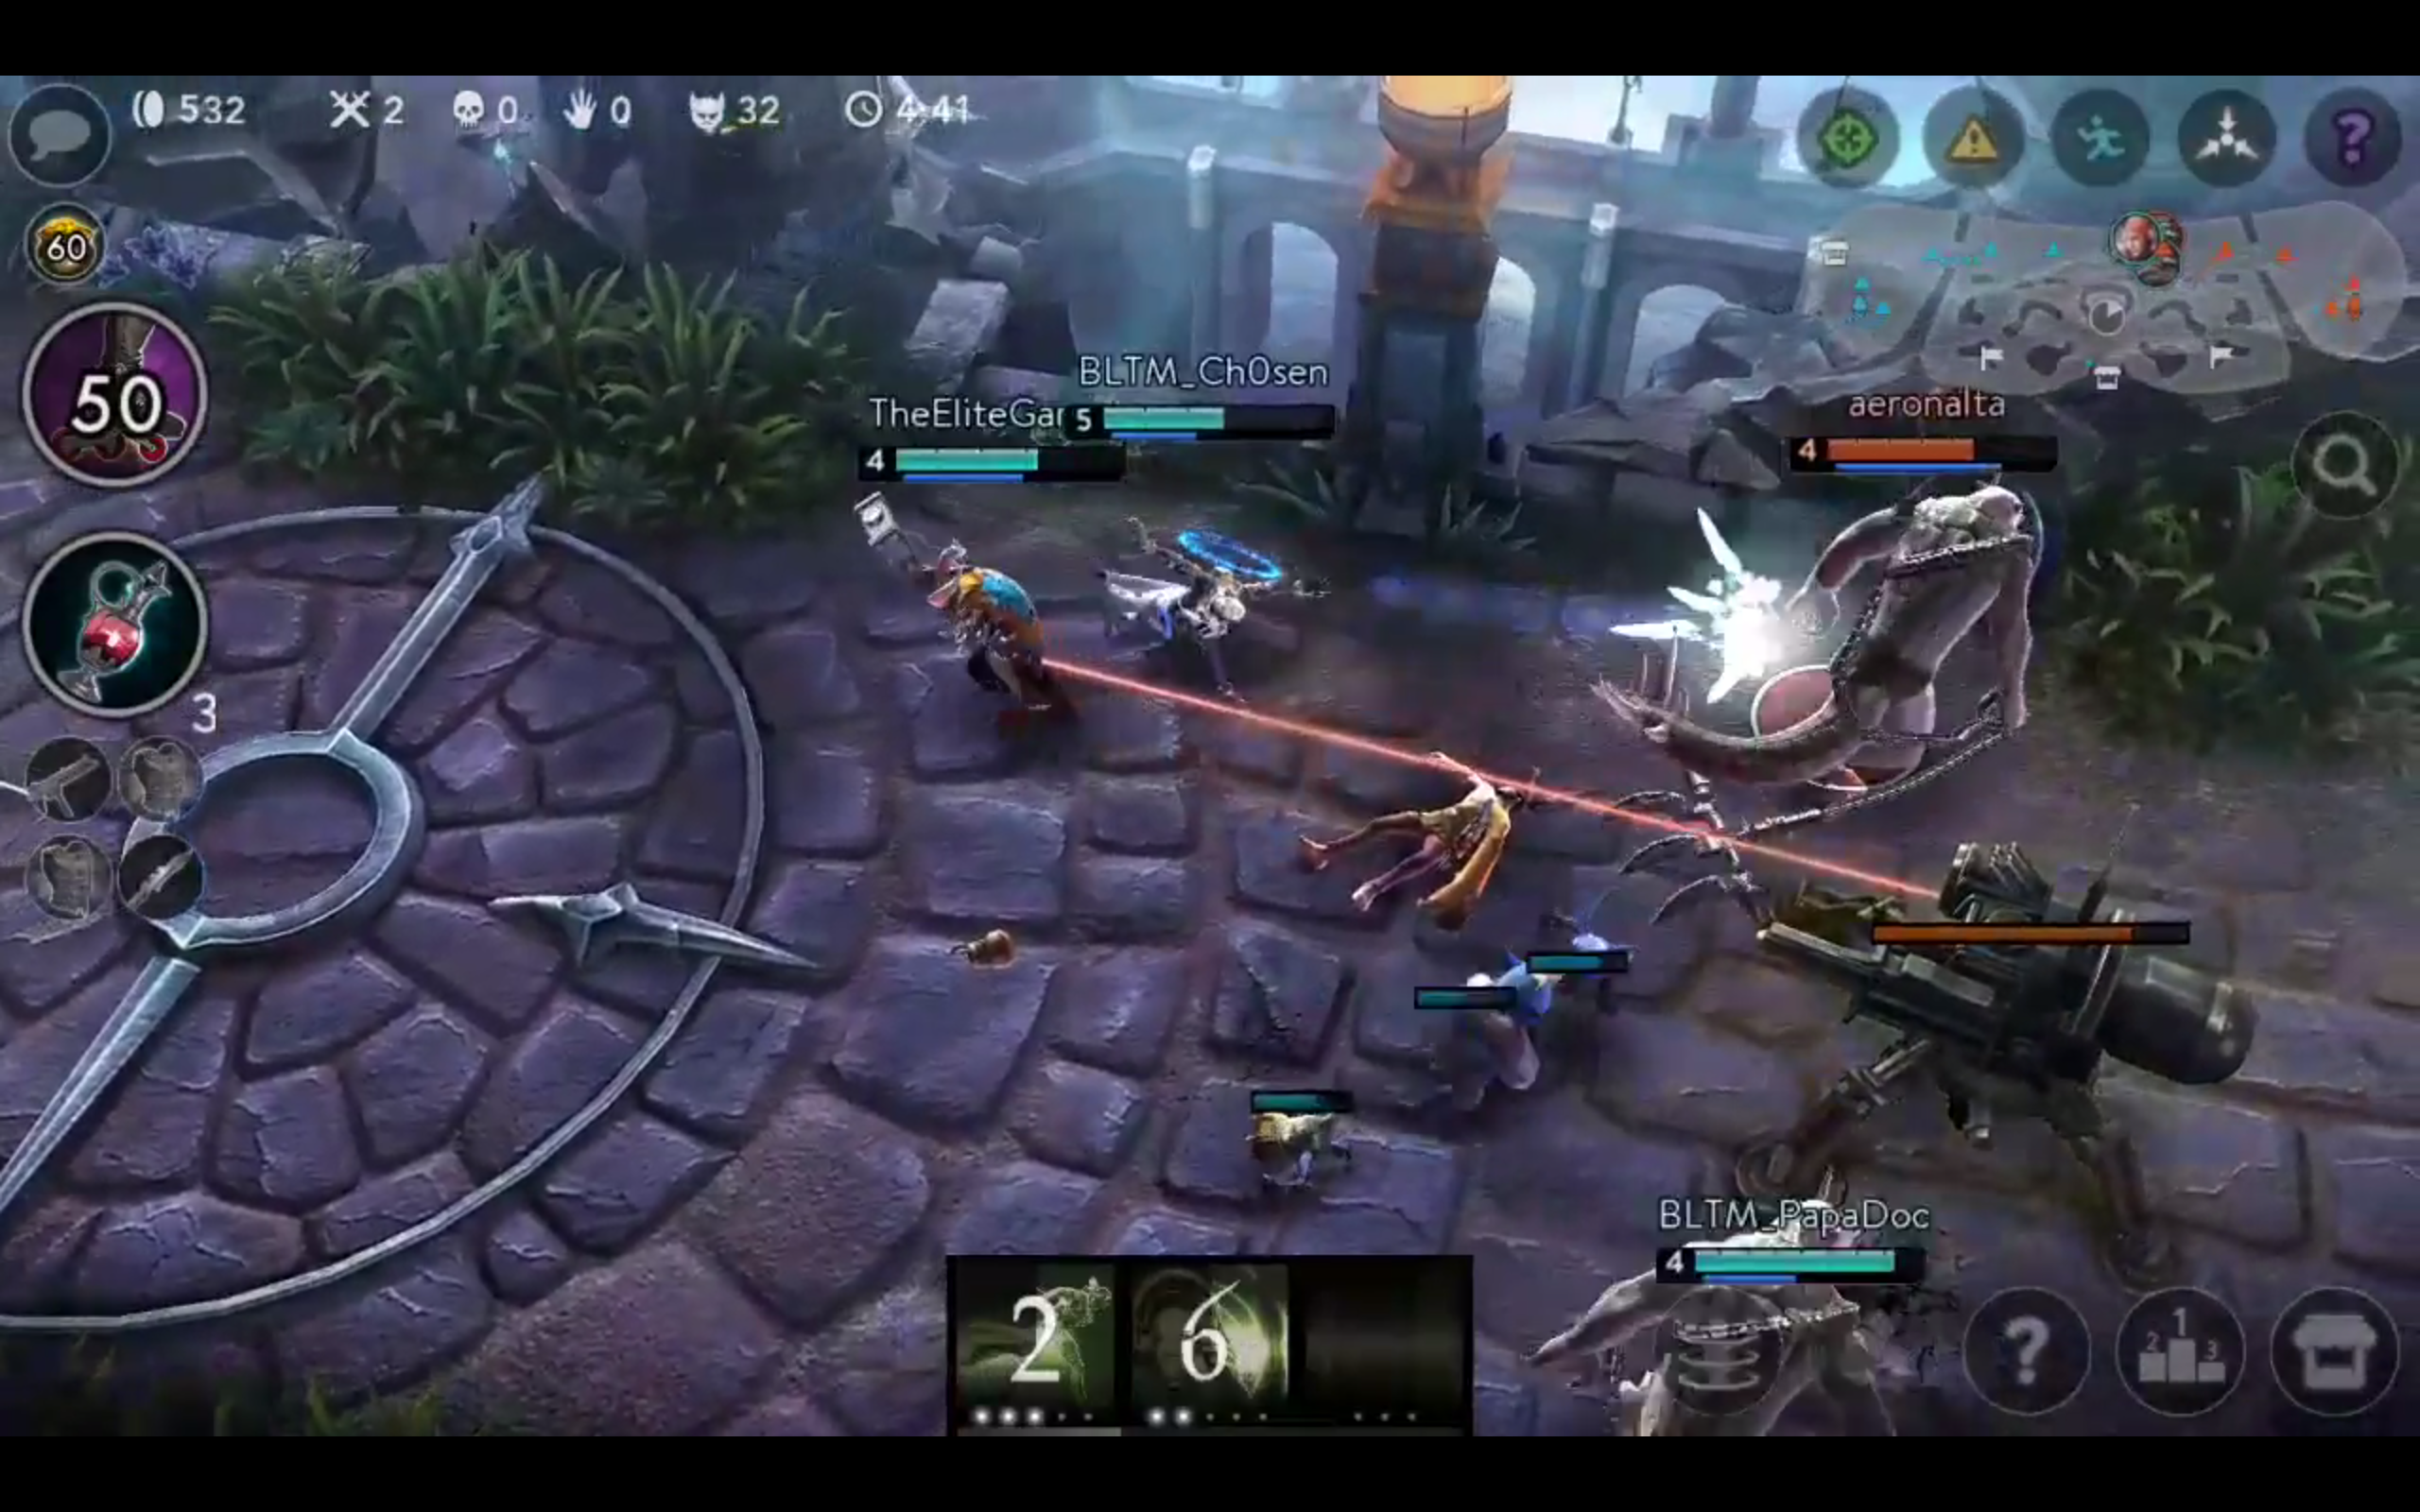
\includegraphics[scale=0.2]{galaxy_s7_edge-vainglory}
		\caption{\emph{Vainglory} ejecutado en un Samsung Galaxy S7 Edge}
		\label{fig:vainglory}
	\end{center}
\end{figure}
